\chapter{Experimental setup}

The exerimental setup was largely adopted from \cite{Hertlein2017}, amendments
made include the \gls{rf} signal source of the \gls{aod} and an additional
photodiode to measure the deflected beam intensity.

\section{Optics}

The optical setup can be dissect into a closed first section that reduces
the power of the $\SI{532}{\nano\meter}$ laser source from $\SI{10}{\watt}$
to below $\SI{2}{\milli\watt}$ and an open second section for beam deflection.
Both sections are connected through a \gls{smf}.

\subsection{Power reduction}
\label{sec:powerbox}

Because of safety concerns the power reduction section is confined into a
visually sealed superstructure. \Cref{fig:powerbox} reveals the inside of the
power reduction box.

\begin{figure}[h]
  \centering
  \includegraphics[width=\textwidth]{standalone/powerbox.pdf}
  \caption{Optical configuration of the power reduction section.}
  \label{fig:powerbox}
\end{figure}

The laser beam leaving the laser source is polarized by a $\lambda/2$ retarder
plate such that the succeeding high power beamsplitter BS can divert the
majority of the beams power into a high power beam dump.
Afterwards mirrors M1 and M2 direct the beam towards the center of a $2:1$
telescope composed of two lenses L1, L2 with focal lengths
$f_1=\SI{100}{\milli\meter}$ and $f_2=\SI{50}{\milli\meter}$.
An \gls{aom} diffracts the laser beam into multiple orders. Mirrors M3, M4
project theses orders onto a pinhole which is configured to intromit only the
the first order deflection. The intensity of the first order is subject to
amplitude modulation apllied to the \gls{aom}.
Finally a tunable $\lambda/2$ retarder plate can be used to couple the beam
polarization with the \gls{smf}.

\subsection{Beam deflection and detection}
\label{sec:deflection}

The section for beam deflection and detection as disclosed in
\cref{fig:deflection} receives the down-powered laser beam from previously
described section by a \gls{smf}. Hereinafter the beam passes a tunable
retarder plate and beam splitter BS1. The tunable retarder plate can be used
to adjust the beam intensity without having to access the power box.
A second polarizer with cube BS2 is used to branch off a part of the beam
to a photodiode PD1 that is positioned to be at the focal point of lens L1.
Photodiode PD1 is connected via a control system with the amplitude
modulation of the \gls{aom} depicted in \cref{fig:powerbox} to stabilize
the laser intensity against i.e. thermal drifts.

\begin{figure}[h]
  \centering
  \includegraphics[width=\textwidth]{standalone/deflection.pdf}
  \caption{Optical configuration of the beam deflection section.}
  \label{fig:deflection}
\end{figure}

For horizontal and vertical beam deflection two \gls{aod}s are used. A $1:1$
telescope comprised of two lenses L2, L3
each with focal length $f_2=f_3=\SI{250}{\milli\meter}$ projects the beam
on a pair of objectives that are built of lenses L4 to L7. The purpose of the
objective pair is to focus the laser on to the atom plane.
Consecutively the laser is reflected by a pair of mirrors M3 and M4 to the
part intended for detection. Lens L8 acts as a camera lens and projects the
beam to infinite focus on to the CCD camera sensor. Cube BS3 forks a portion
of the beam away from the CCD camera on to mirror M5 that guides the beam
towards lens L9 in order to focus the beam onto a second photodiode PD2.

\section{Electronics}

Beforehand we described the optical setups used. Now we want to emphasize
on the electronics how they are integrated into the optical setup.

\subsection{Signal source}

The requirements placed by the two \gls{aod} demand flexible but precise
\gls{rf} sources. Fortunately we can resort to a custom made signal
sources based on the \gls{ad9910} \gls{dds} \cite{AD9910} \gls{ic} that can
operate up to \SI{420}{\mega\hertz} and allows modulation of amplitude,
frequency and phase offset by either a constant value or through a single
digital ramp or playback from a memory sequence.

The signal output of the \gls{dds} is of the form
\begin{equation}
  U(t)=A(t)\sin(2\pi f(t)+\phi(t)).
  \label{eq:dds:signal}
\end{equation}
In the following we will ignore the unsynced phase offset, thus setting
$\phi=0$. In case of the single \gls{dds} which drives the \gls{aom} we
have a constant signal, in that sense we can set $A=1$ and
$f_\text{aom}=\SI{80}{\mega\hertz}$ on \cref{eq:dds:signal}.
In the case of the two \gls{dds} which drive the horizontal and vertical
\gls{aod} we configure the frequency to be controlled by the digital ramp in
order to do a linear frequency sweep from
$f_\text{lower}=\SI{90}{\mega\hertz}$ to
$f_\text{upper}=\SI{110}{\mega\hertz}$, yielding
\begin{align}
  f_\text{aod}(t)
  =
  f_\text{lower} + \frac{f_\text{upper}-f_\text{lower}}{T_\text{duration}}t
\end{align}
wherein $T_\text{duration}>0$ denotes the sweep duration. The amplitude is
controlled by memory playback. Given a discrete set of amplitude values
$A_i\in[0,1]$ with $i=1,\dots,N=1024$ the amplitude of the \gls{aod} can be
formulated as
\begin{align}
  A_\text{aod}(t)
  =\sum^N_{i=1}A_i\mathbb{1}_{B_i}(t)
  &&
  B_i:=\left[iT_\text{interval}, (i+1)T_\text{interval}\right[
\end{align}
wherein $T_\text{interval}>0$ denotes the playback interval and
$\mathbb{1}_{B_i}$ is the characteristic function on the set $B_i$.

So far we have assumed $f_\text{aod}(t)$ to be continous and
$T_\text{interval},T_\text{duration}>0$ to be arbitrary, however the internals
of the \gls{ad9910} impose theoretical restrictions on the possible operating
ranges.

\subsection{Signal amplifier}

We use three signal amplifiers with respective input from the signal sources
to have an output power of about $P=\SI{2}{\watt}$ required by the \gls{aod}s
and \gls{aom} for ideal operation. The used amplifiers offer a second input
for external amplitude modulation. In case of the \gls{aom} we connect this
input with the intensity controller.

\subsection{Intensity controller}

The intensity controller is connected to photodiode PD1 that converts the
laser intensity to an input voltage signal of the controller. Given the
input signal we can configure the controller for a reference input voltage.
The controller will then compare the input voltage with set reference voltage
and output an error signal that is proportional to the deviation of the
input from the reference voltage. The inverted error signal is feed to the
signal amplifier connected with the \gls{aom}.

In one attempt we tried to use the intensity controller to compensate for
frequency dependent intensity changes during frequency sweep of the \gls{aod},
however we found that even slow sweep times of $\SI{2}{\second}$ could not
be balanced, therefore the intensity controller only compensates for slow
intensity shifts caused by thermal stress of the laser source.

The intensity controller has to be connected correctly with photodiode PD1
of the setup as well as signal amplifier of the signal that drives the
\gls{aom}.

\begin{figure}[h]
  \centering
  \includegraphics[height=6cm]{example-image-a}
  \caption{The intensity controller next to the \gls{aom} amplifier.}
  \label{fig:intcontrol}
\end{figure}

The XY can be tuned to set the reference signal.

\subsection{Trigger source}

To syncronize the signal sources, the \gls{ccd} camera and the oscilloscope
it was necessary to design a global trigger source that outputs a rising edge
signal to multiple devices and exposes a network programable interface.

\begin{figure}[h]
  \centering
  \includegraphics[height=6cm]{example-image-a}
  \caption{The trigger source exposes a network programable interface and
  provides enough power to drive four output signals.}
  \label{fig:elec:trig}
\end{figure}
The schematics and board layout can be found in the
\cref{app:electronics:trigger_hub}.

\section{Acousto-Optics}

\subsection{Modulator}
\subsection{Deflector}

\section{Assessment}

With the previously described calibration steps in place we can assess the
final quality of the beam with an image capture of the \gls{ccd} camera in the
aligned setup \cref{sec:deflection}.

\begin{figure}[ht]
  \centering
  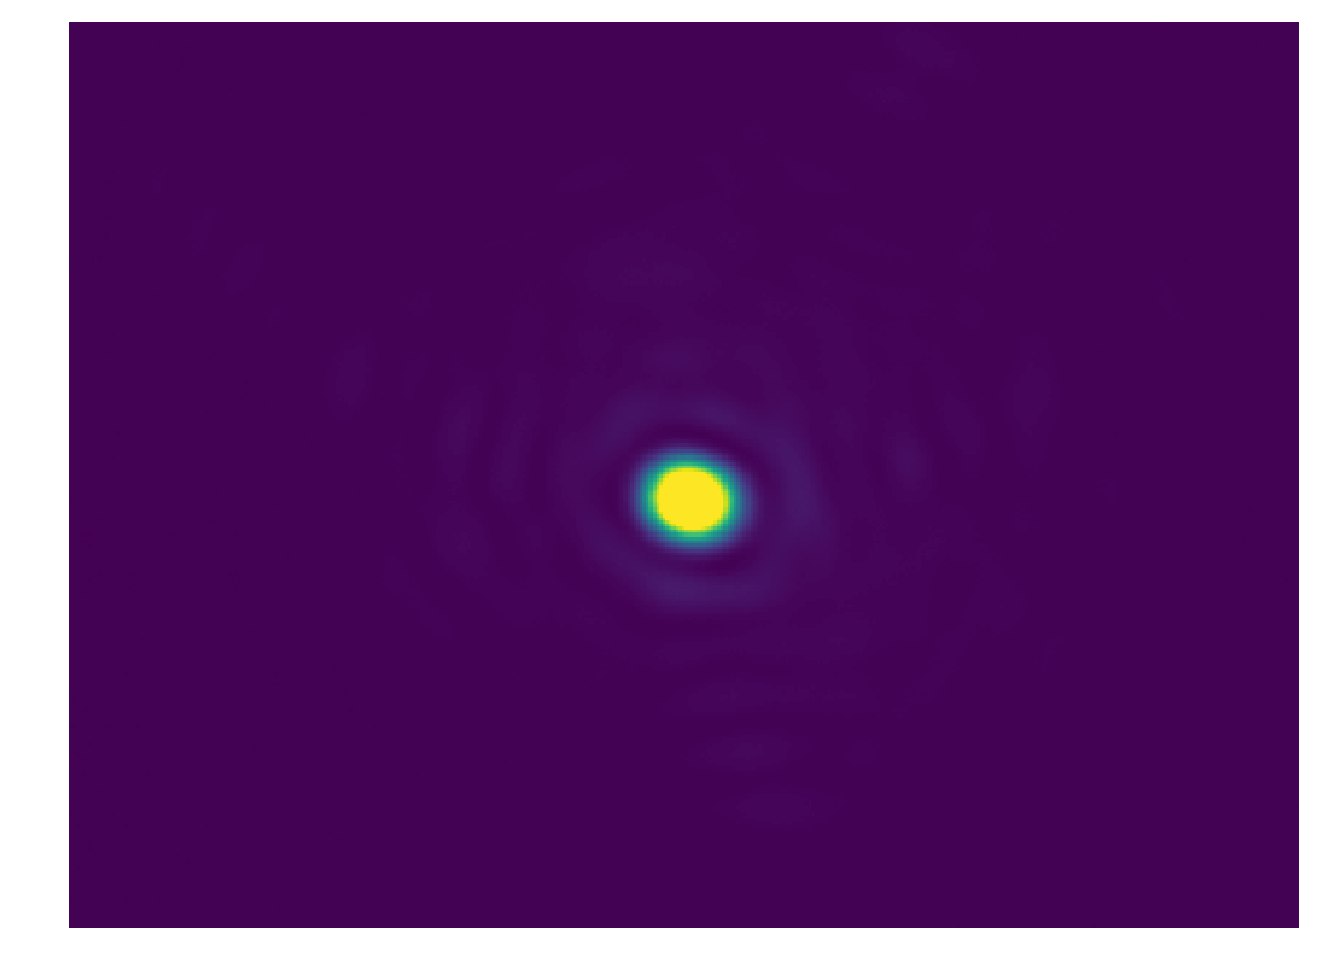
\includegraphics[width=.5\textwidth]{\figuredir{camera/profile2d.pdf}}
  \caption{Image detail from the captured beam with the \gls{ccd} camera.}
  \label{fig:beamprofile:2d}
\end{figure}

The two dimensional beam profile shows the characteristical two dimensional
gaussian distribution with diffraction rings caused by beam clipping at
finite apertures as described in \cite{Hertlein2017}.

\begin{figure}[ht]
  \centering
  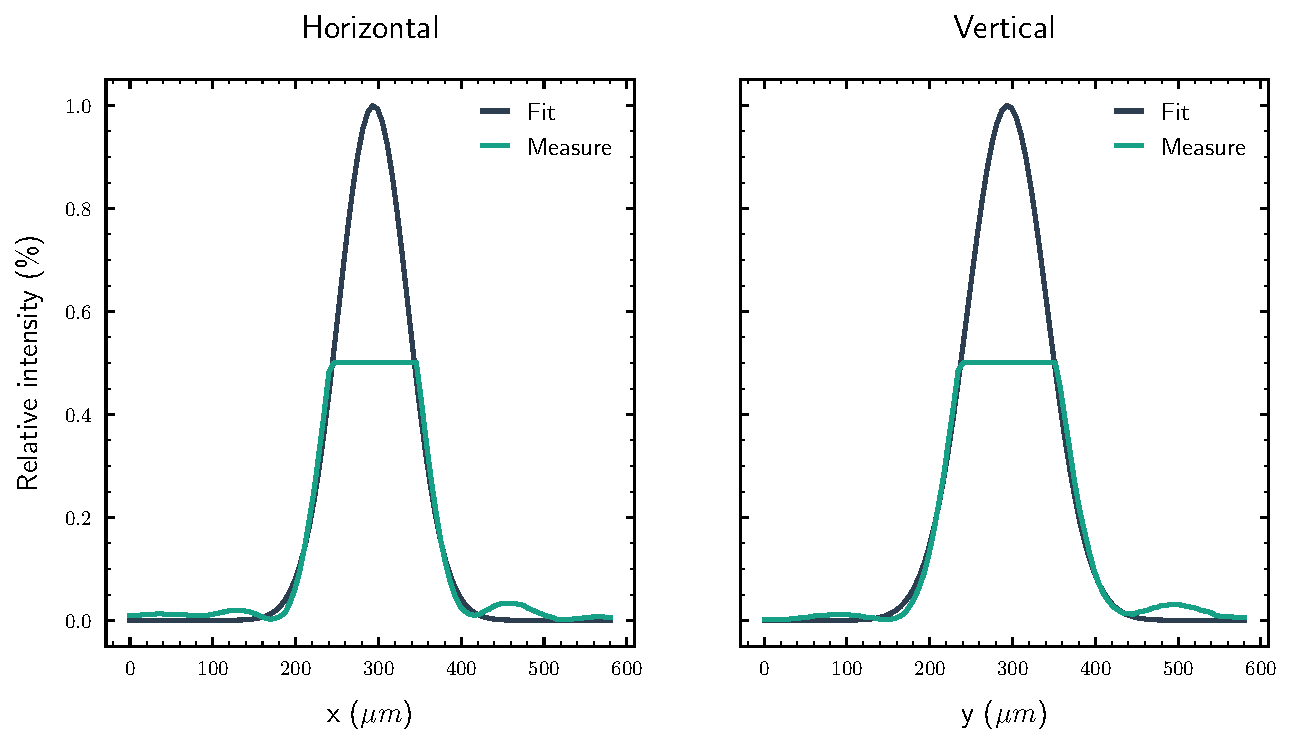
\includegraphics[width=\textwidth]{\figuredir{camera/profile1d.pdf}}
  \caption{1D horizontal and vertical profile extracted from the center of
    the image detail in \cref{fig:beamprofile:2d} with fitted gaussian curve
  and residue.}
  \label{fig:beamprofile:1d}
\end{figure}

By inspecting the one dimensional profiles with fitted gaussian and residue
we again confirm conclusions drawn in \cite{Hertlein2017}. The clipped top
of the measured intensity originates from the saturated pixels of the
\gls{ccd} camera and can be ignored. We further observe a slight assymmetry
at the diffraction rings. Overall the shown profiles can be considered to
confirm a good alignment.
